\documentclass[12pt,a4paper]{article}
\usepackage{fontspec}
\setmainfont{Times New Roman}[Path=C:/Windows/Fonts/,UprightFont=times.ttf,BoldFont=timesbd.ttf,ItalicFont=timesi.ttf,BoldItalicFont=timesbi.ttf]
\usepackage{amsmath,amssymb,amsfonts}
\usepackage[left=1.5cm,right=1.5cm,top=1.5cm,bottom=1.7cm,headheight=17pt]{geometry}
\usepackage{enumitem,array,graphicx,tikz,fancyhdr,needspace,booktabs}
\usetikzlibrary{patterns}

\pagestyle{fancy}
\fancyhf{}
\lhead{\small\textbf{BÀI TẬP VỀ NHÀ TOÁN 12 -- ĐỀ SỐ 2}}
\rhead{\small\textit{Biên soạn: Dương Gia Bảo}}
\rfoot{\small Trang \thepage}
\renewcommand{\headrulewidth}{0.4pt}
\fancypagestyle{firstpage}{\fancyhead{}\renewcommand{\headrulewidth}{0pt}}

\setlength{\parindent}{0pt}
\setlength{\parskip}{3pt}
\setlength{\emergencystretch}{1em}

\setlist[enumerate,1]{label=\textbf{Câu \arabic*:},leftmargin=*,itemsep=6pt,topsep=4pt}

% Macro trắc nghiệm 4 phương án
\newcommand{\bonpa}[4]{\par\nobreak\smallskip\nobreak\noindent
\begin{tabular}{@{}p{0.48\linewidth}p{0.48\linewidth}@{}}
\textbf{A.} #1 & \textbf{B.} #2\\[7pt]
\textbf{C.} #3 & \textbf{D.} #4\end{tabular}}

% Macro khung ô li viết bài làm trực tiếp (kích thước rộng rãi)
\newcommand{\khungOli}[1][5.0cm]{%
  \needspace{2.5cm}%
  \par\nobreak\vspace{4pt}\noindent
  \begin{tikzpicture}
    \pgfmathsetmacro{\gridw}{\linewidth - 1.5pt}
    \draw[step=0.5cm, line width=0.2pt, gray!32] (0,0) grid (\gridw pt, #1);
    \draw[line width=0.6pt, gray!60] (0,0) rectangle (\gridw pt, #1);
    \node[anchor=north east, font=\footnotesize\itshape\color{gray!60}, inner sep=4pt] at (\gridw pt, #1) {Bài làm của học sinh};
  \end{tikzpicture}
  \par\vspace{7pt}
}

\begin{document}
\thispagestyle{firstpage}

\noindent
\begin{minipage}[t]{0.36\textwidth}
    \centering
    {\fontsize{12}{14}\selectfont\textbf{BÀI TẬP VỀ NHÀ}}\\[4pt]
    \textit{Biên soạn: Dương Gia Bảo}\\[6pt]
    \setlength{\fboxrule}{0.8pt}
    \setlength{\fboxsep}{5pt}
    \fbox{\begin{minipage}{0.88\linewidth}
        \centering
        {\fontsize{12}{14}\selectfont\textbf{ÔN TẬP TOÁN 12 -- ĐỀ 2}}
    \end{minipage}}
\end{minipage}\hfill
\begin{minipage}[t]{0.62\textwidth}
    \centering
    {\fontsize{13}{15}\selectfont\textbf{CHUYÊN ĐỀ ÔN TẬP SAU THI GIỮA KÌ I}}\\[3pt]
    {\fontsize{12}{14}\selectfont\textbf{THỐNG KÊ GHÉP NHÓM \& NGUYÊN HÀM -- TÍCH PHÂN}}\\[3pt]
    {\fontsize{11}{13}\selectfont\textit{(Chương trình GDPT 2018 -- Gồm 50 câu)}}
\end{minipage}

\par\vspace{4pt}
\hrule height 0.6pt
\vspace{4pt}
\noindent\textit{Họ và tên học sinh:}\dotfill\hspace{0.8cm}\textit{Lớp:}\makebox[3.2cm]{\dotfill}
\par\vspace{3pt}
\hrule height 0.6pt
\vspace{6pt}

%% ==============================================================
%% PHẦN 1: CHƯƠNG III
%% ==============================================================
\begin{center}
    {\fontsize{13}{15}\selectfont\textbf{PHẦN 1. CHƯƠNG III: CÁC SỐ ĐẶC TRƯNG ĐO MỨC ĐỘ PHÂN TÁN}}\\[2pt]
    {\fontsize{13}{15}\selectfont\textbf{CỦA MẪU SỐ LIỆU GHÉP NHÓM (CÂU 1 -- 15)}}
\end{center}

\subsubsection*{I. TRẮC NGHIỆM NHIỀU LỰA CHỌN (5 CÂU)}

\begin{enumerate}
\item Khi sử dụng khoảng biến thiên $R$ và khoảng tứ phân vị $\Delta_Q$ để đo mức độ phân tán của mẫu số liệu ghép nhóm, khẳng định nào sau đây là đúng?
\bonpa{Cả $R$ và $\Delta_Q$ đều nhạy cảm như nhau với các giá trị ngoại lệ.}{Khoảng tứ phân vị $\Delta_Q$ không bị ảnh hưởng bởi các giá trị bất thường ở hai đầu mút, còn khoảng biến thiên $R$ thì bị ảnh hưởng.}{Khoảng biến thiên $R$ luôn nhỏ hơn khoảng tứ phân vị $\Delta_Q$.}{Khoảng tứ phân vị $\Delta_Q$ chỉ phụ thuộc vào nhóm đầu tiên và nhóm cuối cùng.}

\item Mỗi ngày bác Mạnh đều đi bộ rèn luyện sức khỏe. Quãng đường đi bộ mỗi ngày (đơn vị: km) của bác trong $20$ ngày được thống kê lại ở bảng sau:
\begin{center}
\begin{tabular}{|l|c|c|c|c|c|}
\hline
\textbf{Quãng đường (km)} & $[2{,}7; 3{,}0)$ & $[3{,}0; 3{,}3)$ & $[3{,}3; 3{,}6)$ & $[3{,}6; 3{,}9)$ & $[3{,}9; 4{,}2)$ \\ \hline
\textbf{Số ngày} & $3$ & $6$ & $5$ & $3$ & $3$ \\ \hline
\end{tabular}
\end{center}
Khoảng biến thiên của mẫu số liệu ghép nhóm trên là
\bonpa{$1{,}2$}{$1{,}8$}{$1{,}5$}{$0{,}3$}

\item Một mẫu số liệu ghép nhóm có phương sai bằng $s^2 = 16{,}81$. Độ lệch chuẩn $s$ của mẫu số liệu ghép nhóm đó bằng
\bonpa{$4{,}1$}{$4{,}2$}{$8{,}405$}{$282{,}58$}

\item Trong công thức tính tứ phân vị thứ $k$ ($k \in \{1; 2; 3\}$) của mẫu số liệu ghép nhóm cỡ $n$:
\[
Q_k = u_m + \dfrac{\dfrac{kn}{4} - C}{n_m}(u_{m+1} - u_m),
\]
với $[u_m; u_{m+1})$ là nhóm chứa $Q_k$, đại lượng $C$ biểu thị điều gì?
\bonpa{Tần số của nhóm chứa $Q_k$.}{Giá trị đại diện của nhóm chứa $Q_k$.}{Tổng tần số của các nhóm từ nhóm chứa $Q_k$ trở đi.}{Tổng tần số tích lũy của các nhóm đứng trước nhóm chứa $Q_k$.}

\item Thống kê chiều cao (đơn vị: cm) của $40$ học sinh lớp 12B thu được bảng ghép nhóm sau:
\begin{center}
\begin{tabular}{|l|c|c|c|c|c|}
\hline
\textbf{Chiều cao (cm)} & $[150; 155)$ & $[155; 160)$ & $[160; 165)$ & $[165; 170)$ & $[170; 175)$ \\ \hline
\textbf{Số học sinh} & $4$ & $9$ & $15$ & $8$ & $4$ \\ \hline
\end{tabular}
\end{center}
Nhóm chứa tứ phân vị thứ nhất $Q_1$ của mẫu số liệu ghép nhóm trên là
\bonpa{$[150; 155)$}{$[155; 160)$}{$[160; 165)$}{$[165; 170)$}
\end{enumerate}

\subsubsection*{II. TRẢ LỜI NGẮN (10 CÂU) -- HỌC SINH TRÌNH BÀY LỜI GIẢI VÀO KHUNG Ô LI}

\begin{enumerate}[start=6]
\item Một công ty bất động sản thực hiện cuộc khảo sát $500$ khách hàng xem họ có nhu cầu mua nhà ở mức giá nào (đơn vị: triệu đồng/$\text{m}^2$) để chuẩn bị dự án khu đô thị mới. Kết quả được ghi lại ở bảng sau:
\begin{center}
\begin{tabular}{|l|c|c|c|c|c|}
\hline
\textbf{Mức giá (triệu đồng/$\text{m}^2$)} & $[10; 14)$ & $[14; 18)$ & $[18; 22)$ & $[22; 26)$ & $[26; 30)$ \\ \hline
\textbf{Số khách hàng} & $75$ & $105$ & $197$ & $80$ & $43$ \\ \hline
\end{tabular}
\end{center}
Công ty ưu tiên xây dựng phân khúc nhà tầm trung hướng tới $50\%$ số khách hàng ở khoảng giữa của bảng phân phối (từ $Q_1$ đến $Q_3$). Tính khoảng tứ phân vị $\Delta_Q$ (làm tròn kết quả đến hàng phần mười, đơn vị triệu đồng/$\text{m}^2$).
\khungOli[5.5cm]

\item Dựa vào bảng số liệu ghép nhóm về quãng đường đi bộ mỗi ngày trong $20$ ngày của bác Mạnh ở \textbf{Câu 2}, hãy tính phương sai $s^2$ của mẫu số liệu ghép nhóm đó (làm tròn kết quả đến hàng phần trăm).
\khungOli[5.5cm]

\item Điểm thi thử tốt nghiệp THPT môn Toán của $40$ học sinh lớp 12A được thống kê trong bảng số liệu ghép nhóm sau:
\begin{center}
\begin{tabular}{|l|c|c|c|c|c|}
\hline
\textbf{Điểm số} & $[5; 6)$ & $[6; 7)$ & $[7; 8)$ & $[8; 9)$ & $[9; 10)$ \\ \hline
\textbf{Số học sinh} & $4$ & $10$ & $14$ & $8$ & $4$ \\ \hline
\end{tabular}
\end{center}
Tính độ lệch chuẩn $s$ của mẫu số liệu ghép nhóm trên (làm tròn kết quả đến hàng phần trăm).
\khungOli[5.5cm]

\item Thống kê thời gian sử dụng thiết bị điện tử ngoài giờ học (đơn vị: giờ/tuần) của $50$ sinh viên cho kết quả ở bảng sau:
\begin{center}
\begin{tabular}{|l|c|c|c|c|c|}
\hline
\textbf{Thời gian (giờ)} & $[5; 10)$ & $[10; 15)$ & $[15; 20)$ & $[20; 25)$ & $[25; 30)$ \\ \hline
\textbf{Số sinh viên} & $6$ & $x$ & $18$ & $y$ & $4$ \\ \hline
\end{tabular}
\end{center}
Biết rằng số trung bình của mẫu số liệu ghép nhóm là $\bar{x} = 17{,}3$ giờ. Tìm $x, y$ và tính giá trị biểu thức $T = 2x + y$.
\khungOli[5.5cm]

\item Kiểm tra tuổi thọ (tính bằng nghìn giờ) của một lô gồm $60$ bóng đèn LED thu được bảng ghép nhóm sau:
\begin{center}
\begin{tabular}{|l|c|c|c|c|c|}
\hline
\textbf{Tuổi thọ (nghìn giờ)} & $[10; 12)$ & $[12; 14)$ & $[14; 16)$ & $[16; 18)$ & $[18; 20)$ \\ \hline
\textbf{Số bóng đèn} & $8$ & $15$ & $22$ & $10$ & $5$ \\ \hline
\end{tabular}
\end{center}
Tính khoảng tứ phân vị $\Delta_Q$ của mẫu số liệu ghép nhóm trên (làm tròn kết quả đến hàng phần trăm).
\khungOli[5.5cm]

\item Khảo sát mức lương khởi điểm (tính theo triệu đồng/tháng) của $80$ sinh viên vừa tốt nghiệp khối ngành kỹ thuật thu được bảng số liệu:
\begin{center}
\begin{tabular}{|l|c|c|c|c|c|}
\hline
\textbf{Mức lương (triệu đồng)} & $[8; 10)$ & $[10; 12)$ & $[12; 14)$ & $[14; 16)$ & $[16; 18)$ \\ \hline
\textbf{Số sinh viên} & $12$ & $24$ & $28$ & $12$ & $4$ \\ \hline
\end{tabular}
\end{center}
Để thuộc nhóm $25\%$ sinh viên có mức lương cao nhất trong mẫu khảo sát thì mức lương tối thiểu phải đạt bao nhiêu triệu đồng (tức tìm $Q_3$, làm tròn kết quả đến hàng phần trăm)?
\khungOli[5.0cm]

\item Một xưởng cơ khí kiểm tra đường kính (đơn vị: mm) của $32$ trục thép do Máy I sản xuất và thu được bảng ghép nhóm:
\begin{center}
\begin{tabular}{|l|c|c|c|c|}
\hline
\textbf{Đường kính (mm)} & $[20{,}0; 20{,}2)$ & $[20{,}2; 20{,}4)$ & $[20{,}4; 20{,}6)$ & $[20{,}6; 20{,}8)$ \\ \hline
\textbf{Số trục thép} & $6$ & $10$ & $10$ & $6$ \\ \hline
\end{tabular}
\end{center}
Biết rằng Máy II sản xuất cùng loại trục thép trên có độ lệch chuẩn là $s_{\text{II}} = 0{,}25\text{ mm}$. Tính tỉ số $\dfrac{s_{\text{II}}}{s_{\text{I}}}$ giữa độ lệch chuẩn của Máy II và Máy I.
\khungOli[5.5cm]

\item Tốc độ di chuyển (đơn vị: km/h) của $50$ xe ô tô khi đi qua một trạm kiểm soát giao thông được ghi lại như sau:
\begin{center}
\begin{tabular}{|l|c|c|c|c|c|}
\hline
\textbf{Tốc độ (km/h)} & $[40; 50)$ & $[50; 60)$ & $[60; 70)$ & $[70; 80)$ & $[80; 90)$ \\ \hline
\textbf{Số ô tô} & $5$ & $12$ & $20$ & $10$ & $3$ \\ \hline
\end{tabular}
\end{center}
Tính phương sai $s^2$ của mẫu số liệu ghép nhóm trên.
\khungOli[5.5cm]

\item Thống kê số cuốn sách đọc được trong một năm của $40$ học sinh thu được bảng ghép nhóm có độ dài các nhóm không bằng nhau như sau:
\begin{center}
\begin{tabular}{|l|c|c|c|c|}
\hline
\textbf{Số sách (cuốn)} & $[0; 2)$ & $[2; 4)$ & $[4; 8)$ & $[8; 12)$ \\ \hline
\textbf{Số học sinh} & $5$ & $11$ & $16$ & $8$ \\ \hline
\end{tabular}
\end{center}
Tính khoảng tứ phân vị $\Delta_Q$ của mẫu số liệu ghép nhóm trên (làm tròn kết quả đến hàng phần trăm).
\khungOli[5.5cm]

\item Lượng mưa trung bình mỗi tháng (đơn vị: mm) tại một trạm quan trắc khí tượng trong $24$ tháng được thống kê ở bảng sau:
\begin{center}
\begin{tabular}{|l|c|c|c|c|c|}
\hline
\textbf{Lượng mưa (mm)} & $[50; 100)$ & $[100; 150)$ & $[150; 200)$ & $[200; 250)$ & $[250; 300)$ \\ \hline
\textbf{Số tháng} & $4$ & $6$ & $8$ & $4$ & $2$ \\ \hline
\end{tabular}
\end{center}
Tính độ lệch chuẩn $s$ của mẫu số liệu ghép nhóm trên (làm tròn kết quả đến hàng phần mười).
\khungOli[5.5cm]
\end{enumerate}

\newpage
%% ==============================================================
%% PHẦN 2: CHƯƠNG IV
%% ==============================================================
\begin{center}
    {\fontsize{13}{15}\selectfont\textbf{PHẦN 2. CHƯƠNG IV: NGUYÊN HÀM VÀ TÍCH PHÂN (CÂU 16 -- 50)}}
\end{center}

\subsubsection*{I. TRẮC NGHIỆM NHIỀU LỰA CHỌN (15 CÂU)}

\begin{enumerate}[start=16]
\item Tìm họ nguyên hàm của hàm số $f(x) = x^3 - \dfrac{2}{x^2} + 1$ trên khoảng $(0; +\infty)$.
\bonpa{$\dfrac{x^4}{4} - \dfrac{2}{x} + x + C$}{$\dfrac{x^4}{4} + \dfrac{2}{x} + x + C$}{$3x^2 + \dfrac{4}{x^3} + C$}{$\dfrac{x^4}{4} + \dfrac{1}{x} + x + C$}

\item Họ nguyên hàm của hàm số $f(x) = \cos(3x - 1) + \dfrac{1}{\cos^2 x}$ là
\bonpa{$\dfrac{1}{3}\sin(3x-1) + \tan x + C$}{$-\dfrac{1}{3}\sin(3x-1) + \tan x + C$}{$3\sin(3x-1) + \tan x + C$}{$\dfrac{1}{3}\sin(3x-1) - \cot x + C$}

\item Họ nguyên hàm của hàm số $f(x) = \sin^2 x$ là
\bonpa{$\dfrac{x}{2} + \dfrac{\sin 2x}{4} + C$}{$\dfrac{x}{2} - \dfrac{\sin 2x}{2} + C$}{$\dfrac{x}{2} - \dfrac{\sin 2x}{4} + C$}{$\dfrac{\sin^3 x}{3} + C$}

\item Biết $\int f(x)\,\mathrm{d}x = \mathrm{e}^{2x} + x^2 + C$. Khẳng định nào sau đây là đúng?
\bonpa{$f(x) = \mathrm{e}^{2x} + 2x$}{$f(x) = \dfrac{1}{2}\mathrm{e}^{2x} + \dfrac{x^3}{3}$}{$f(x) = 2\mathrm{e}^{2x} + x^2$}{$f(x) = 2\mathrm{e}^{2x} + 2x$}

\item Gọi $F(x)$ là một nguyên hàm của hàm số $f(x) = \mathrm{e}^x + 2x$ thỏa mãn $F(0) = 3$. Giá trị của $F(1)$ bằng
\bonpa{$\mathrm{e} + 2$}{$\mathrm{e} + 3$}{$\mathrm{e} + 4$}{$\mathrm{e} + 1$}

\item Cho hàm số $y = f(x)$ liên tục trên $\mathbb{R}$ và có một nguyên hàm là $F(x)$. Biết rằng $F(1) = 9$ và $F(2) = 5$. Giá trị của tích phân $\int_1^2 f(x)\,\mathrm{d}x$ bằng
\bonpa{$14$}{$-4$}{$45$}{$4$}

\item Cho $\int_0^3 f(x)\,\mathrm{d}x = 6$ và $\int_0^3 g(x)\,\mathrm{d}x = -2$. Tính tích phân $I = \int_0^3 [3f(x) - 2g(x)]\,\mathrm{d}x$.
\bonpa{$22$}{$14$}{$20$}{$18$}

\item Giá trị của tích phân $I = \int_0^3 |x - 1|\,\mathrm{d}x$ bằng
\bonpa{$\dfrac{3}{2}$}{$2$}{$\dfrac{5}{2}$}{$\dfrac{7}{2}$}

\item Tính tích phân $I = \int_0^1 x\mathrm{e}^{x^2}\,\mathrm{d}x$.
\bonpa{$\dfrac{\mathrm{e} - 1}{2}$}{$\mathrm{e} - 1$}{$\dfrac{\mathrm{e} + 1}{2}$}{$\dfrac{\mathrm{e}}{2}$}

\item Giá trị của tích phân $I = \int_1^{\mathrm{e}} \ln x\,\mathrm{d}x$ bằng
\bonpa{$\mathrm{e}$}{$\mathrm{e} - 1$}{$0$}{$1$}

\item Diện tích $S$ của hình phẳng giới hạn bởi hai đồ thị hàm số $y = x^2$ và $y = x + 2$ là
\bonpa{$\dfrac{7}{2}$}{$\dfrac{9}{2}$}{$5$}{$\dfrac{11}{2}$}

\item Một vật thể nằm giữa hai mặt phẳng $x = 0$ và $x = 2$. Khi cắt vật thể bởi mặt phẳng vuông góc với trục $Ox$ tại điểm có hoành độ $x$ ($0 \le x \le 2$), thiết diện thu được là một tam giác đều có độ dài cạnh bằng $x$. Thể tích của vật thể đó là
\bonpa{$\dfrac{\sqrt{3}}{3}$}{$\dfrac{4\sqrt{3}}{3}$}{$\dfrac{2\sqrt{3}}{3}$}{$2\sqrt{3}$}

\item Quay hình phẳng giới hạn bởi đường thẳng $y = 2x$ và parabol $y = x^2$ quanh trục hoành $Ox$. Thể tích $V$ của khối tròn xoay tạo thành bằng
\bonpa{$\dfrac{64\pi}{15}$}{$\dfrac{32\pi}{15}$}{$\dfrac{16\pi}{15}$}{$\dfrac{64}{15}$}

\item Một vật bắt đầu chuyển động với vận tốc ban đầu $v_0 = 2\text{ m/s}$ và gia tốc biến thiên theo thời gian là $a(t) = 6t$ ($\text{m/s}^2$). Vận tốc của vật tại thời điểm $t = 4$ giây là
\bonpa{$48\text{ m/s}$}{$26\text{ m/s}$}{$52\text{ m/s}$}{$50\text{ m/s}$}

\item Một hồ chứa nước đang cạn được bơm nước vào với tốc độ chảy vào tại thời điểm $t$ phút ($t \ge 0$) được cho bởi $V'(t) = 3t^2 + 4$ ($\text{m}^3$/phút). Lượng nước được bơm vào hồ trong $3$ phút đầu tiên (từ $t = 0$ đến $t = 3$) bằng
\bonpa{$31\text{ m}^3$}{$35\text{ m}^3$}{$39\text{ m}^3$}{$27\text{ m}^3$}
\end{enumerate}

\subsubsection*{II. TRẢ LỜI NGẮN (20 CÂU) -- HỌC SINH TRÌNH BÀY LỜI GIẢI VÀO KHUNG Ô LI}

\begin{enumerate}[start=31]
\item Cho hàm số $f(x)$ xác định trên $(0; +\infty)$ thỏa mãn $f'(x) = \dfrac{3}{2\sqrt{x}} + 2x$ và $f(1) = 5$. Tính giá trị của $f(4)$.
\khungOli[4.8cm]

\item Cho hàm số $f(x) = \dfrac{x^2 + 2x + 4}{x + 1}$. Gọi $F(x)$ là một nguyên hàm của $f(x)$ trên khoảng $(-1; +\infty)$ thỏa mãn $F(0) = 1$. Biết rằng $F(1) = \dfrac{a}{b} + c\ln 2$, trong đó $a, b, c \in \mathbb{Z}^+$ và $\dfrac{a}{b}$ là phân số tối giản. Tính giá trị của $a + b + c$.
\khungOli[5.5cm]

\item Biết nguyên hàm $\int (2x + 3)\ln x\,\mathrm{d}x = (x^2 + 3x)\ln x - \dfrac{a}{b}x^2 - cx + C$, với $a, b, c \in \mathbb{Z}^+$ và $\dfrac{a}{b}$ là phân số tối giản. Tính giá trị của $a + b + c$.
\khungOli[5.5cm]

\item Gọi $F(x)$ là một nguyên hàm của hàm số $f(x) = \sin^4 x \cos x$ thỏa mãn $F(0) = 0$. Tính giá trị của $F\!\left(\dfrac{\pi}{2}\right)$.
\khungOli[4.5cm]

\item Cho hàm số $f(x) = \begin{cases} 3x^2 - 1 & \text{khi } x \ge 1 \\ 2x & \text{khi } x < 1 \end{cases}$. Tính giá trị của tích phân $I = \int_0^2 f(x)\,\mathrm{d}x$.
\khungOli[4.8cm]

\item Tính tích phân $I = \int_1^{\mathrm{e}} \dfrac{\sqrt{1 + 3\ln x}}{x}\,\mathrm{d}x$. Biết kết quả là phân số tối giản $\dfrac{a}{b}$ với $a, b \in \mathbb{Z}^+$. Tính $a + b$.
\khungOli[5.5cm]

\item Biết tích phân $I = \int_0^{\pi} (x + 1)\sin x\,\mathrm{d}x = a\pi + b$ với $a, b \in \mathbb{Z}$. Tính giá trị của biểu thức $P = a^2 + b^2$.
\khungOli[5.5cm]

\item Biết tích phân $I = \int_0^1 \dfrac{3x + 5}{(x + 1)(x + 2)}\,\mathrm{d}x = a\ln 2 + b\ln 3$ với $a, b \in \mathbb{Z}$. Tính giá trị của biểu thức $T = a + 2b$.
\khungOli[5.5cm]

\item Biết tích phân $I = \int_0^{\ln 2} \dfrac{\mathrm{e}^x}{\mathrm{e}^x + 1}\,\mathrm{d}x = \ln\!\left(\dfrac{a}{b}\right)$ với $a, b$ là các số nguyên dương nguyên tố cùng nhau. Tính giá trị của $a + b$.
\khungOli[4.8cm]

\item Tìm số thực $m > 1$ thỏa mãn đẳng thức tích phân $\int_1^m \left(3x^2 - \dfrac{4}{x^2}\right)\,\mathrm{d}x = 5$.
\khungOli[5.0cm]

\item Tại một địa điểm, trong khoảng thời gian $12$ giờ, nhiệt độ tại thời điểm $t$ (tính bằng giờ, $0 \le t \le 12$) được mô hình hóa bởi hàm số $T(t) = 25 + 4t - \dfrac{1}{3}t^2$ ($^\circ\text{C}$). Tính nhiệt độ trung bình trong $12$ giờ đó, biết nhiệt độ trung bình bằng $\dfrac{1}{12}\int_0^{12} T(t)\,\mathrm{d}t$.
\khungOli[5.0cm]

\item Giả sử lợi nhuận biên (tính theo triệu đồng trên tấn) của một sản phẩm được tính theo công thức $P'(x) = 18 - 0{,}04x$, trong đó $P(x)$ (triệu đồng) là lợi nhuận thu được khi bán $x$ tấn sản phẩm. Tính phần lợi nhuận tăng thêm (đơn vị: triệu đồng) khi sản lượng bán tăng từ $50$ tấn lên $100$ tấn.
\khungOli[5.0cm]

\item Một bồn chứa đang chứa đầy $3000$ lít nước thì bị rò rỉ. Tốc độ nước chảy khỏi bồn tại thời điểm $t$ phút kể từ lúc bị rò rỉ được cho bởi công thức $r(t) = 160 - 2t$ (lít/phút). Hỏi sau $15$ phút đầu tiên, trong bồn còn lại bao nhiêu lít nước?
\khungOli[5.0cm]

\item Một chất điểm chuyển động trên trục thẳng đứng với vận tốc tại thời điểm $t$ giây ($0 \le t \le 6$) được cho bởi:
\[
v(t) = \begin{cases} 3t^2 & \text{khi } 0 \le t \le 2 \\ 12 - 2(t - 2) & \text{khi } 2 < t \le 6 \end{cases}\quad (\text{đơn vị: m/s}).
\]
Tính tổng quãng đường (mét) chất điểm đi được trong $6$ giây đầu tiên.
\khungOli[5.5cm]

\item Tính diện tích hình phẳng giới hạn bởi parabol $y = x^2 - 4x + 3$ và đường thẳng $y = x - 1$.
\khungOli[5.0cm]

\item Một cánh cổng của một tòa nhà có dạng hình parabol như hình vẽ dưới đây, gồm hai phần: phần hai cánh cửa hình chữ nhật $CDEF$ và phần hoa văn trang trí (phần gạch chéo). Biết chiều cao cổng $GH = 4\text{ m}$, chiều rộng chân cổng $AB = 4\text{ m}$ và $AC = BD = 0{,}9\text{ m}$. Tính diện tích phần hoa văn trang trí (đơn vị: $\text{m}^2$, làm tròn kết quả đến hàng phần trăm).
\begin{center}
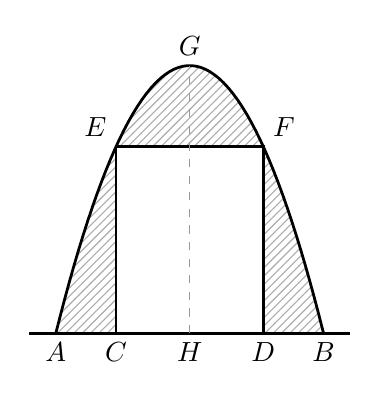
\begin{tikzpicture}[scale=0.85]
  % Cổng parabol y = 4 - x^2, x in [-2, 2]
  \fill[pattern=north east lines, pattern color=gray!65] plot[domain=-2:2, samples=60] (\x, {4 - \x*\x}) -- (2,0) -- (-2,0) -- cycle;
  % Khoét phần cửa hình chữ nhật CDEF: x in [-1.1, 1.1], y in [0, 2.79]
  \fill[white] (-1.1, 0) rectangle (1.1, 2.79);
  % Vẽ đường parabol và các đoạn thẳng
  \draw[line width=1pt] plot[domain=-2:2, samples=60] (\x, {4 - \x*\x});
  \draw[line width=1pt] (-2.4, 0) -- (2.4, 0);
  \draw[line width=0.9pt] (-1.1, 0) -- (-1.1, 2.79) -- (1.1, 2.79) -- (1.1, 0);
  \draw[dashed, gray!80] (0, 0) -- (0, 4);
  \draw[dashed, gray!80] (0, 0) -- (0, 2.79);
  % Các điểm
  \node[below] at (-2, 0) {$A$};
  \node[below] at (2, 0) {$B$};
  \node[below] at (-1.1, 0) {$C$};
  \node[below] at (1.1, 0) {$D$};
  \node[above left] at (-1.1, 2.79) {$E$};
  \node[above right] at (1.1, 2.79) {$F$};
  \node[above] at (0, 4) {$G$};
  \node[below] at (0, 0) {$H$};
\end{tikzpicture}
\end{center}
\khungOli[6.0cm]

\item Một vật thể giới hạn bởi hai mặt phẳng $x = 0$ và $x = 3$. Khi cắt vật thể bởi mặt phẳng vuông góc với trục $Ox$ tại điểm có hoành độ $x$ ($0 \le x \le 3$), thiết diện thu được là một hình chữ nhật có hai kích thước là $x$ và $\sqrt{9 - x^2}$. Tính thể tích $V$ của vật thể đó.
\khungOli[5.2cm]

\item Khi thiết kế một chậu cây trang trí bằng phần mềm mô phỏng 3D, người ta quay hình phẳng giới hạn bởi đồ thị hàm số $y = \sqrt{x} + 2$, trục hoành và hai đường thẳng $x = 0, x = 4$ quanh trục $Ox$. Biết đơn vị trên mỗi trục tọa độ là đề-xi-mét ($\text{dm}$). Tính thể tích của chậu cây theo đơn vị $\text{dm}^3$ (lấy $\pi \approx 3{,}1416$ và làm tròn kết quả đến hàng phần mười).
\khungOli[5.5cm]

\item Một chi tiết máy được chế tạo bằng cách quay hình phẳng giới hạn bởi đường cong $y = x^2 - 4x + 5$, trục hoành $Ox$ và hai đường thẳng $x = 1, x = 4$ quanh trục $Ox$. Biết đơn vị trên các trục tọa độ là $\text{cm}$. Tính thể tích của chi tiết máy đó theo đơn vị $\text{cm}^3$ (lấy $\pi \approx 3{,}1416$ và làm tròn kết quả đến hàng đơn vị).
\khungOli[5.8cm]

\item Một chỏm cầu chứa nước có thể tích bằng thể tích khối tròn xoay sinh ra khi quay hình phẳng giới hạn bởi đường cong $y = \sqrt{25 - x^2}$, trục hoành $Ox$ và hai đường thẳng $x = 2, x = 5$ quanh trục $Ox$. Gọi thể tích này là $V$. Hãy tìm giá trị của $\dfrac{V}{\pi}$.
\khungOli[5.0cm]
\end{enumerate}

\end{document}
